\section{Flow-Sinkhorn for Graph Wasserstein--1}\label{sec:applications}
The same abstract rate applies to dense balanced transport (Appendix~\ref{app-app:sinkhorn-ot}) and to the sparse graph formulation developed here. Their entropy penalties act on different variables, so identical $\gamma$ values do not define identical regularized problems. Our numerical comparisons should be read with this distinction in mind.

\paragraph{Graph and flow conventions.}\label{subsec-w1-graphs}
Let $G=(V,E)$ be a connected undirected graph represented by both orientations of each edge, with no self-loops. Put $n=|V|\geq2$, $p=|E|$, and $0<W_{\min}\leq W_{ij}=W_{ji}\leq W_{\max}$ on $E$. Let $b_1,b_2$ be probability vectors and $q=b_1-b_2$. The entry $f_{ij}$ transports mass from $j$ to $i$, so $(Bf)_i=(f^\top\mathbf1-f\mathbf1)_i$ is outgoing minus incoming flow. If $D_{ij}$ denotes the weighted shortest-path distance, then the transport cost with ground matrix $D$ equals
\begin{equation}\label{eq-W1-flow}
 W_1(b_1,b_2)=\min\{\langle W,f\rangle:f\in\mathbb R_+^E,\ Bf=q\}.
\end{equation}
Routing a coupling along shortest paths and decomposing a feasible flow into paths and cycles prove this equivalence. Positive edge costs allow cycles to be discarded at an optimum. Let $\Dhop$ be the maximum minimum \emph{number} of edges in a path and $\Dweight=\max_{ij}D_{ij}$ the weighted diameter; these are different quantities.

\paragraph{A normalized lifted split.}\label{subsec-splitting-constr}
Fix a positive reference $z\in\mathbb R_{++}^E$ and $Z=\sum_Ez_{ij}$. We regularize~\eqref{eq-W1-flow} by $\gamma\KL(f|z)$. Duplicating the flow gives the exactly equivalent problem
\begin{equation}\label{eq-W1-flow-lifted}
 \min_{(f,g)\in\mathcal C_1\cap\mathcal C_2}
 \frac{\langle W,f\rangle+\langle W,g\rangle}{2}
 +\frac{\gamma}{2}\{\KL(f|z)+\KL(g|z)\},\quad
 \mathcal C_1=\{-f\mathbf1+g^\top\mathbf1=q\},\quad
 \mathcal C_2=\{f=g\}.
\end{equation}
Nonnegativity of both flows is implicit. The generic parameters are $\bar C=(W/2,W/2)$, $\bar z=(z,z)$, and $\theta=\gamma/2$. Thus $\bar C/\theta=(W/\gamma,W/\gamma)$, and the Gibbs initialization is $(K,K)$ with $K=z e^{-W/\gamma}$. The factor $1/2$ changes values, not the projection sequence. A strictly positive feasible flow exists: add a positive symmetric circulation on every edge to any feasible flow. The lifted operators, their adjoint, and all gauge conventions are given in Appendix~\ref{app-app:w1-proofs}.

\begin{proposition}[Closed-form projections]\label{prop:graphw1-projection-closed-form}
For strictly positive $f,g$ on $E$, let $r_i=\sum_j f_{ij}$ and $c_i=\sum_j g_{ji}$. The $\mathcal C_1$ projection is $(f',g')=(\diag(s)f,g\diag(s)^{-1})$, where $s_i>0$ solves $r_is_i-c_i/s_i=-q_i$, namely $s_i=(\sqrt{q_i^2+4r_ic_i}-q_i)/(2r_i)$. The $\mathcal C_2$ projection of $(f',g')$ is $(h,h)$ with $h_{ij}=\sqrt{f'_{ij}g'_{ij}}$.
\end{proposition}
Consequently a full sweep starting at $(h,h)$ is
\begin{equation}\label{eq:proj-sinkh-flow}
 h^{+}_{ij}=h_{ij}\sqrt{s_i/s_j},\qquad h^{(0)}=K.
\end{equation}
The row/column sums and edgewise updates take $O(p)$ operations and storage. Appendix~\ref{app-app:w1-proofs} derives the projections, including the sign convention.

\begin{proposition}[Potential implementation]\label{prop:graphw1-flow-sinkhorn-update}
At each full step there is a potential $v\in\mathbb R^V$ such that $h_{ij}=K_{ij}e^{(v_j-v_i)/\gamma}$, initialized by $v=0$. Define $\alpha_i^+=\gamma\log\sum_jK_{ij}e^{v_j/\gamma}$ and $\alpha_i^-=\gamma\log\sum_jK_{ji}e^{-v_j/\gamma}$. Then~\eqref{eq:proj-sinkh-flow} is equivalent to
\begin{equation}\label{eq:v-update-stable}
 v_i^+=\frac{v_i}{2}+\frac{\alpha_i^+-\alpha_i^-}{4}
 +\frac\gamma2\arsinh\left(\frac{q_i}{2}
 e^{-(\alpha_i^++\alpha_i^-)/(2\gamma)}\right).
\end{equation}
\end{proposition}
Log-sum-exp evaluation of the $\alpha_i^\pm$ avoids direct kernel underflow. The inverse-hyperbolic-sine term also needs a log-domain evaluation at extreme arguments; Appendix~\ref{app-app:w1-proofs} supplies one. These algebraic rewritings reduce overflow risk, but do not constitute a finite-precision error theorem. The generic dual is used with $\theta=\gamma/2$, not $\gamma$, when reporting physical transport values. At a full step this is the directly evaluable scalar $F_\gamma^{\rm flow}(v)=\langle q,v\rangle+\gamma Z-\gamma\sum_{ij\in E}K_{ij}e^{(v_j-v_i)/\gamma}$.

\paragraph{Convergence analysis.}\label{sec:conv-analysis-flow}
\begin{theorem}[Explicit graph optimal-value complexity]\label{thm:graphw1-complexity}
Under the graph assumptions above, let $L_z=\|\log z\|_\infty$, $z_{\min}=\min_Ez$, and choose any nonnegative feasible comparison flow $\bar f$. Define
\begin{align}\label{eq:graph-constants}
 M_\gamma&=\frac{\langle W,\bar f\rangle+\gamma\KL(\bar f|z)}{W_{\min}},&
 H_\gamma&=|\log M_\gamma|+L_z+\frac{2W_{\max}}\gamma,\notag\\
 U_\gamma&=\Dhop(W_{\max}+\gamma H_\gamma),&
 X_\gamma&=\frac{2\|q\|_1U_\gamma}{\gamma}+2Ze^{-W_{\min}/\gamma}.
\end{align}
Here $M_\gamma>0$, and $X_\gamma$ bounds the \emph{lifted} mass $\|f\|_1+\|g\|_1$, including half-steps. Set $M_0=(n-1)\|q\|_1/2$ and $B_0=Z+M_0\log\max\{1,M_0/z_{\min}\}$, interpreting the second term as zero when $M_0=0$. For $\gamma=\varepsilon/(2B_0)$ and
$K\geq\max\{1,\lceil256 B_0X_\gamma U_\gamma^2/\varepsilon^2\rceil\}$,
the physical lifted dual value at step $K$ differs from $W_1(b_1,b_2)$ by at most $\varepsilon$. The iteration cost is $O(pK)$. For fixed graph, reference, and measures this is $O(p\varepsilon^{-3})$ as $\varepsilon\downarrow0$, with no condition relating $p$ and $\varepsilon$.
\end{theorem}
\paragraph{Proof sketch.}
The graph block maps are order preserving and commute with constant translations. Hence their composition is non-expansive in the variation seminorm $\|v\|_{\rm Var}=(\max v-\min v)/2$. A path argument gives $\kappa_1\leq\Dhop$. Positive costs bound the optimal flow mass by $M_\gamma$; the identity $f^\star_{ij}f^\star_{ji}=z_{ij}z_{ji}e^{-2W_{ij}/\gamma}$ then gives $H_\gamma$. The dual helper with cost $W/2$ and parameter $\theta=\gamma/2$ gives $U_\gamma$. Since the second right-hand side is zero, $\langle(q,0),(v,U)\rangle\leq\|q\|_1U_\gamma$, and the primal helper gives~\eqref{eq:graph-constants}. Finally, $\|A\|_{1\to1}=2$, the lifted bias envelope is $2B_0$, and Theorem~\ref{thm:approx-linprog} yields the stated count. Appendix~\ref{app-app:w1-proofs} proves every graph-specific input and explains how to construct $\bar f$.

\paragraph{What the guarantee does and does not measure.}
An iterate satisfying $f=g$ need not yet satisfy $Bf=q$. Routing a residual of total positive mass $\|q-Bf\|_1/2$ along shortest paths gives a feasible correction of cost at most $\Dweight\|q-Bf\|_1/2$. This is useful for a posteriori certification, but is not included in the theorem's optimal-value bound. Opposite directed flows can be cancelled without changing divergence, decreasing linear cost; they are not zero in the entropic optimum. The plots below use neither this cancellation nor potential debiasing. Comparisons with exact network-flow solvers would require a different accuracy protocol. Such solvers are particularly relevant at high accuracy; the present experiments do not establish a speed advantage over them.

\paragraph{Numerical experiments.}
We compare flow-Sinkhorn with vanilla Sinkhorn on the dense geodesic cost matrix, using the previously recorded CPU and GPU runs in Figures~\ref{fig:bench-overview-small} and~\ref{fig:bench-line-gpu-scaling}. The implementations use double precision. The measured quantity is a dual-potential diagnostic, \emph{not} a flow error or the theorem's dual-objective gap. For the centered potential $\widetilde v=v-n^{-1}(\sum_i v_i)\mathbf1$ and a chosen centered LP-optimal potential $\widetilde v^\star$, the recorded statistic is
\begin{equation}\label{eq:benchmark-error}
 e(t)=\min_{s:\ t_s\leq t}\ \min_{\sigma\in\{-1,1\}}
 \frac{\|\widetilde v^{(s)}-\sigma\widetilde v^\star\|_2}
 {\|\widetilde v^\star\|_2}.
\end{equation}
The benchmark code includes the sign alignment to accommodate potential conventions; a sign flip is not an additional gauge of a fixed transport problem. The displayed instances have nonzero denominator. On graphs where the LP potential is nonunique beyond its additive constant, this error depends on the selected reference optimizer. It is therefore an empirical diagnostic, not a distance to the whole optimal set and not a certified cost error. Curves show the best recorded error, so their monotonicity does not assert monotonicity of potential distances along the actual iterates.

The benchmark configurations are:
\begin{itemize}[leftmargin=1.2em,itemsep=2pt,topsep=3pt,parsep=0pt]
\item \textbf{Line.} A path with $n=80$ vertices, $p=158$ directed edges of unit weight, and uniform source and target measures supported on the first and last $m=6$ vertices. GPU runs also use $(n,m)=(160,12),(320,24)$. Here $D_{ij}=|i-j|$ and $W_1=\sum_{i=1}^{n-1}|\sum_{j\leq i}q_j|$, so both ground distances and the reference cost can be computed without Floyd--Warshall or an LP solver.
\item \textbf{Delaunay.} A cloud of $n=140$ points in the unit square, Delaunay edges with Euclidean weights, and uniform measures on $m=7$ points near the upper-left and lower-right corners. The realized edge count depends on the triangulation.
\item \textbf{Single cell.} Waddington-OT single-cell RNA-seq measurements of mouse embryonic fibroblast reprogramming toward pluripotency~\citep{schiebinger2019optimal}. We subsample $60$ cells at each of days $0,0.5,1,1.5$, yielding $n=240$ vertices in a $30$-dimensional PCA representation. A symmetrized $4$-nearest-neighbor graph, with connectivity repair when necessary, carries Euclidean edge costs. Blue and red measures are uniform over the initial and final sampled time points. Flow on this cell-state graph is an illustrative transport proxy for reprogramming trajectories, not a validated reconstruction of lineage or fate, and does not replace the temporal/growth model of Waddington-OT.
\end{itemize}
Graph renderings aggregate the two directed entries on an undirected edge as $f_{ij}+f_{ji}$, retain high-magnitude edges for the orange overlay, and draw the underlying graph in gray. Source and target supports are blue and red. CPU plots use common time and error axes for both methods. GPU line experiments use an NVIDIA Quadro RTX 4000 (8 GB); the public drivers also provide a device switch. These are finite-precision benchmark implementations, including their stabilization and relaxation choices, rather than a test of the exact-arithmetic constants in the theorem.

The aim is to illustrate approach to an unregularized reference across regularization strengths, not compare contraction rates for the same regularized functional: the two methods penalize entropy on different variables. Larger $\gamma$ can give a rapid initial improvement and an earlier bias plateau; smaller $\gamma$ can reduce that bias at higher numerical cost. For machine learning, non-vanishing regularization often improves stability or generalization, so approaching the unregularized solution fastest is not necessarily the relevant downstream objective. An extensive task-based evaluation or comparison with exact flow solvers is beyond these experiments. The figures retain the historical runs; their caption ranges must not be confused with newer screening defaults in the benchmark scripts.

\begin{figure}[htbp]
\centering
\begin{minipage}{0.3\linewidth}\centering
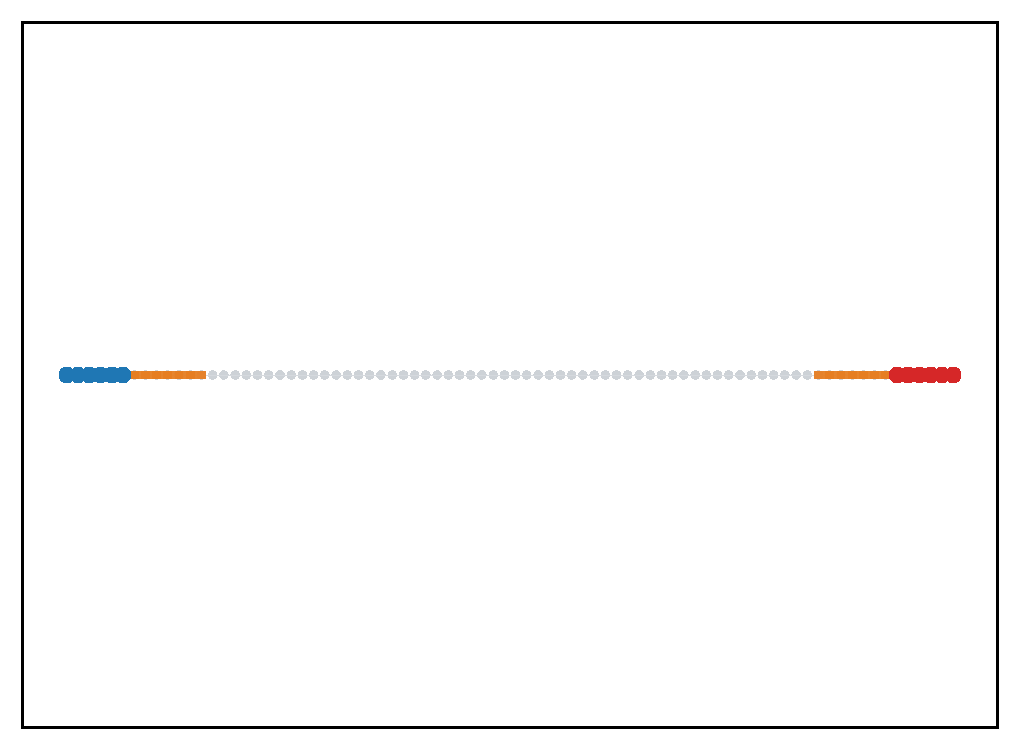
\includegraphics[width=\linewidth]{figures/benchmark-small-line-graph.pdf}
\end{minipage}\hfill
\begin{minipage}{0.3\linewidth}\centering
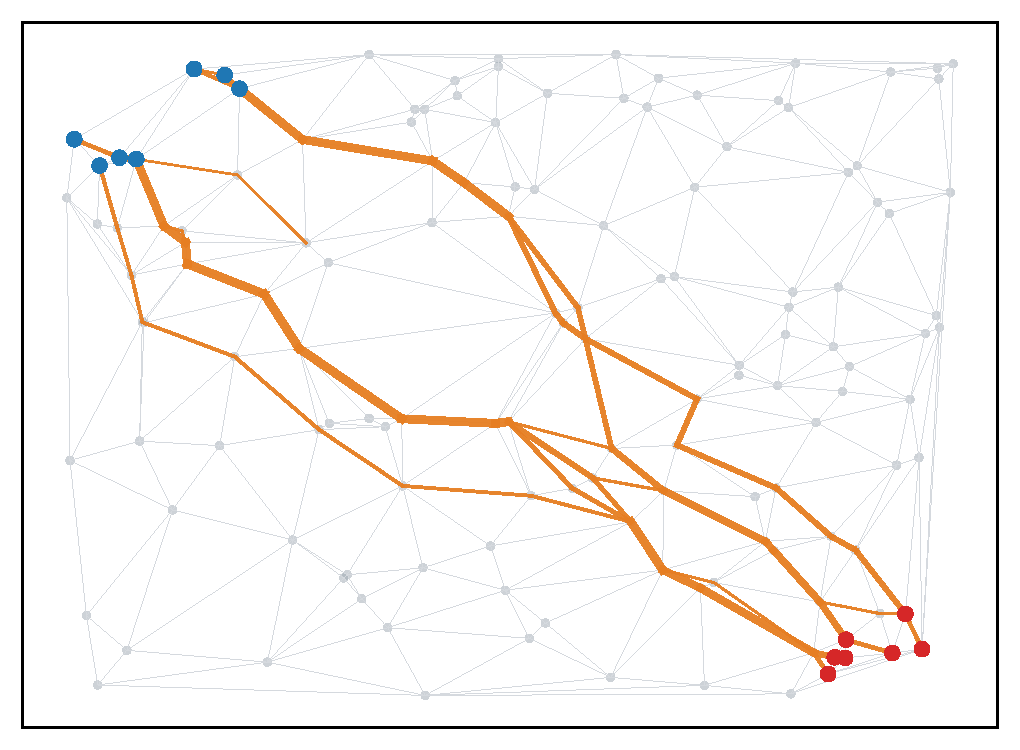
\includegraphics[width=\linewidth]{figures/benchmark-small-delaunay-graph.pdf}
\end{minipage}\hfill
\begin{minipage}{0.3\linewidth}\centering
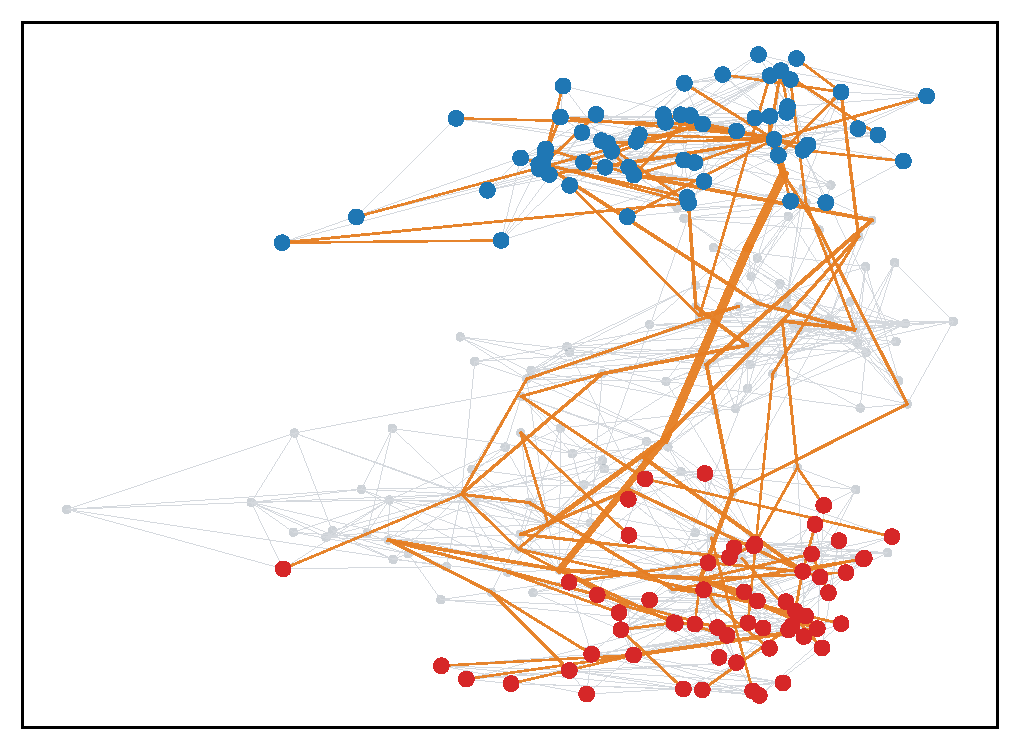
\includegraphics[width=\linewidth]{figures/benchmark-small-singlecell-graph.pdf}
\end{minipage}
% \medskip
\begin{minipage}{0.32\linewidth}\centering
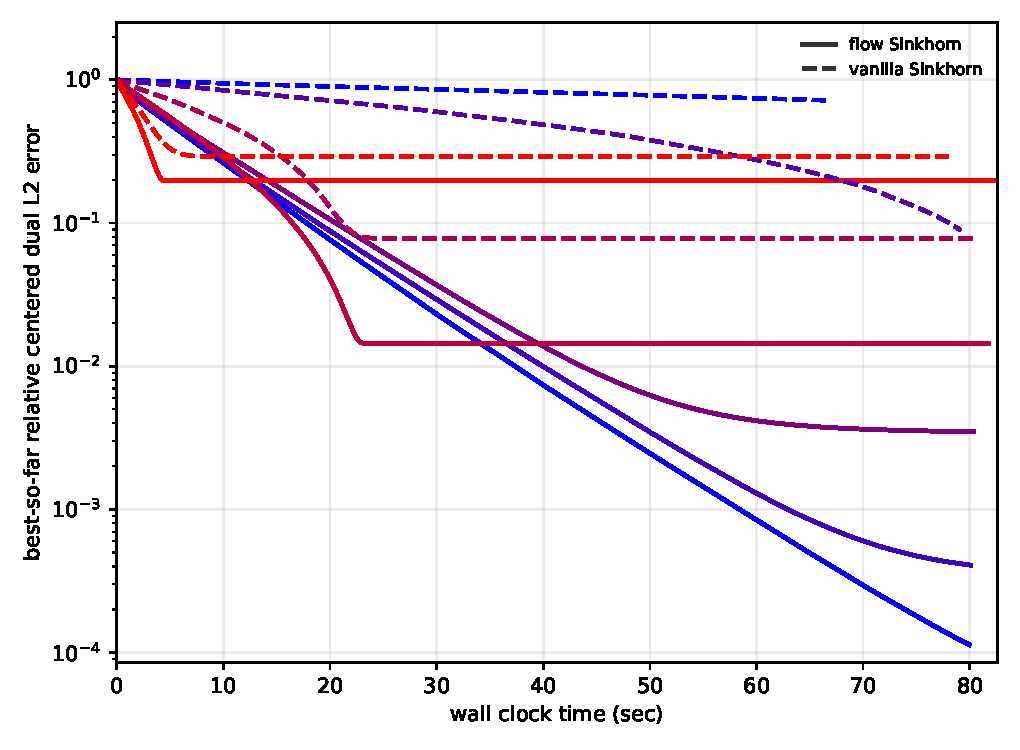
\includegraphics[width=\linewidth]{figures/benchmark-small-line-convergence.pdf}
\end{minipage}\hfill
\begin{minipage}{0.32\linewidth}\centering
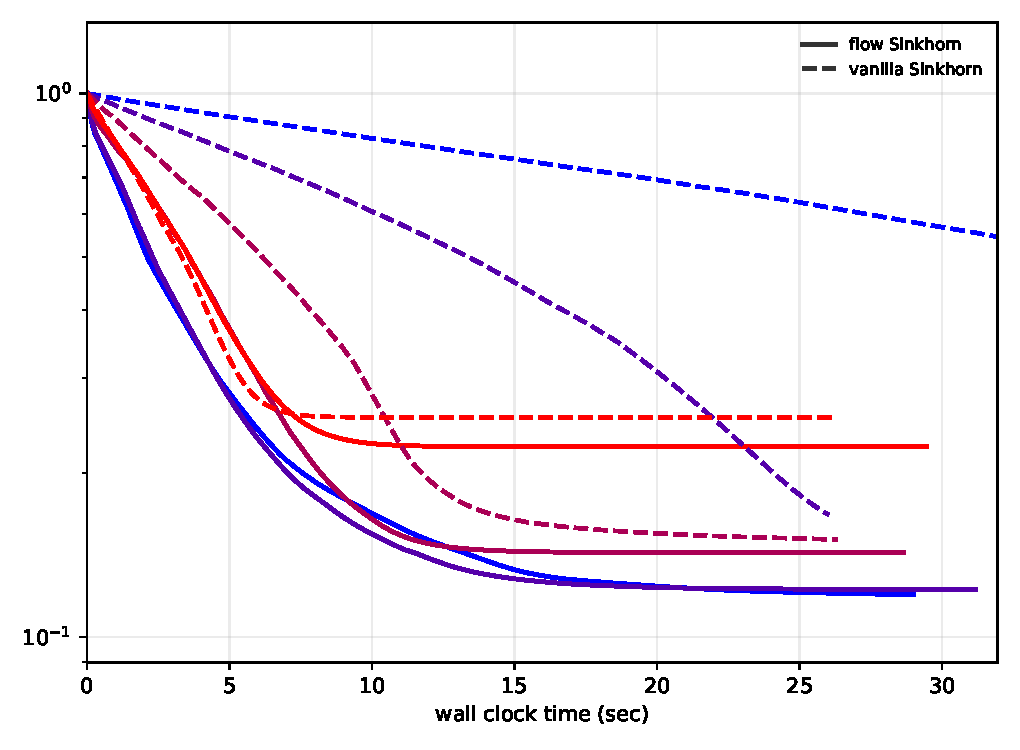
\includegraphics[width=\linewidth]{figures/benchmark-small-delaunay-convergence.pdf}
\end{minipage}\hfill
\begin{minipage}{0.32\linewidth}\centering
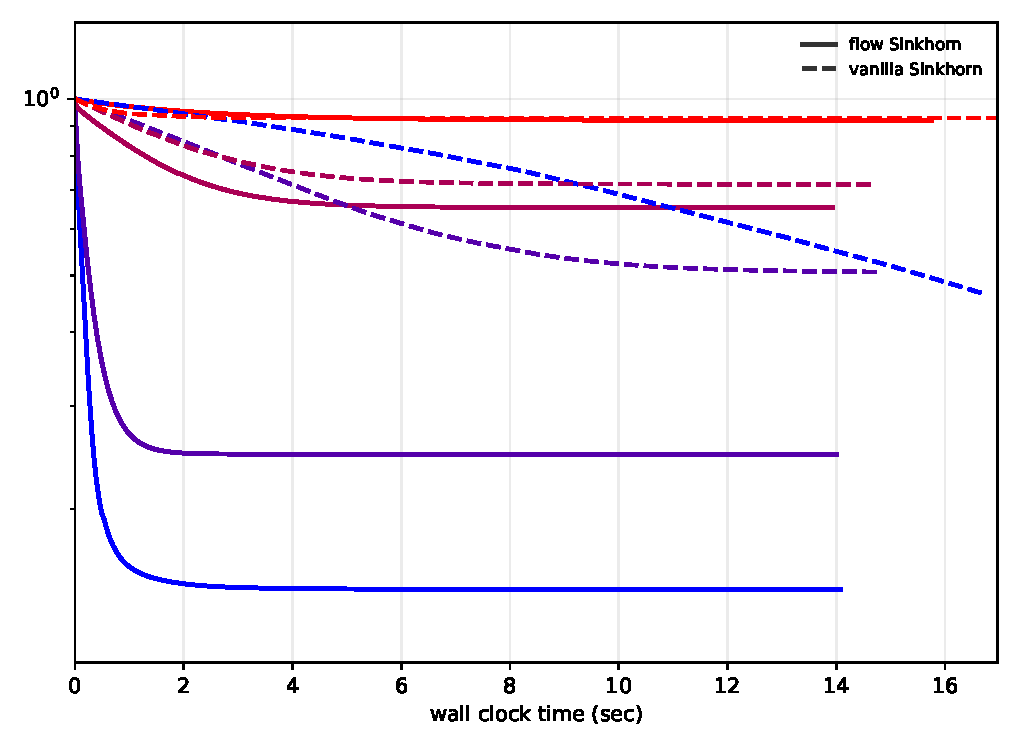
\includegraphics[width=\linewidth]{figures/benchmark-small-singlecell-convergence.pdf}
\end{minipage}\vspace{-2mm}
\caption{Top row: benched graph together with the flow $f$ (line graph, planar Delaunay, single cell). Bottom row: best-so-far relative centered dual-potential error $e(t)$, defined in the text, against wall-clock time. Flow Sinkhorn is plain and vanilla Sinkhorn is dashed; colors encode $\gamma$ from blue (small) to red (large).
Gamma ranges are: line (flow $\gamma\in[10^{-3},5]$, vanilla $\gamma\in[10^{-1},1]$), Delaunay (flow $\gamma\in[9\times10^{-4},9\times10^{-3}]$, vanilla $\gamma\in[9\times10^{-4},9\times10^{-3}]$), single-cell (flow $\gamma\in[3\times10^{-1},9]$, vanilla $\gamma\in[1,5]$).}
\label{fig:bench-overview-small}
\end{figure}

\begin{figure}[htbp]
\centering
\begin{minipage}{0.32\linewidth}\centering
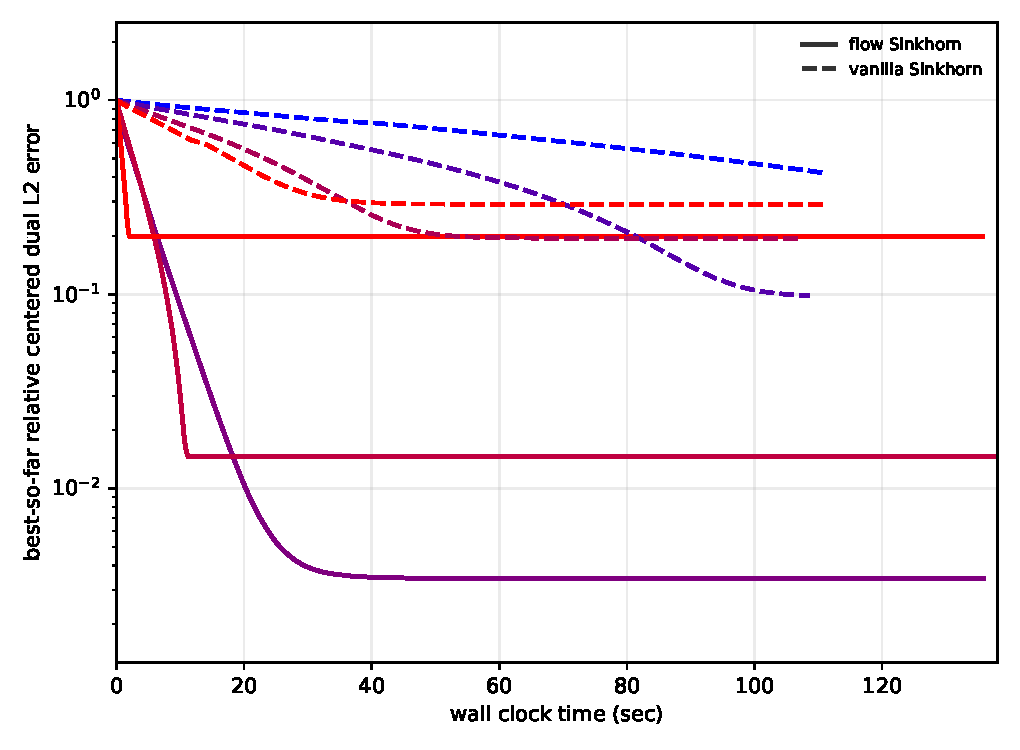
\includegraphics[width=\linewidth]{figures/benchmark-gpu-small-half-tuned-line-convergence.pdf}
\end{minipage}\hfill
\begin{minipage}{0.32\linewidth}\centering
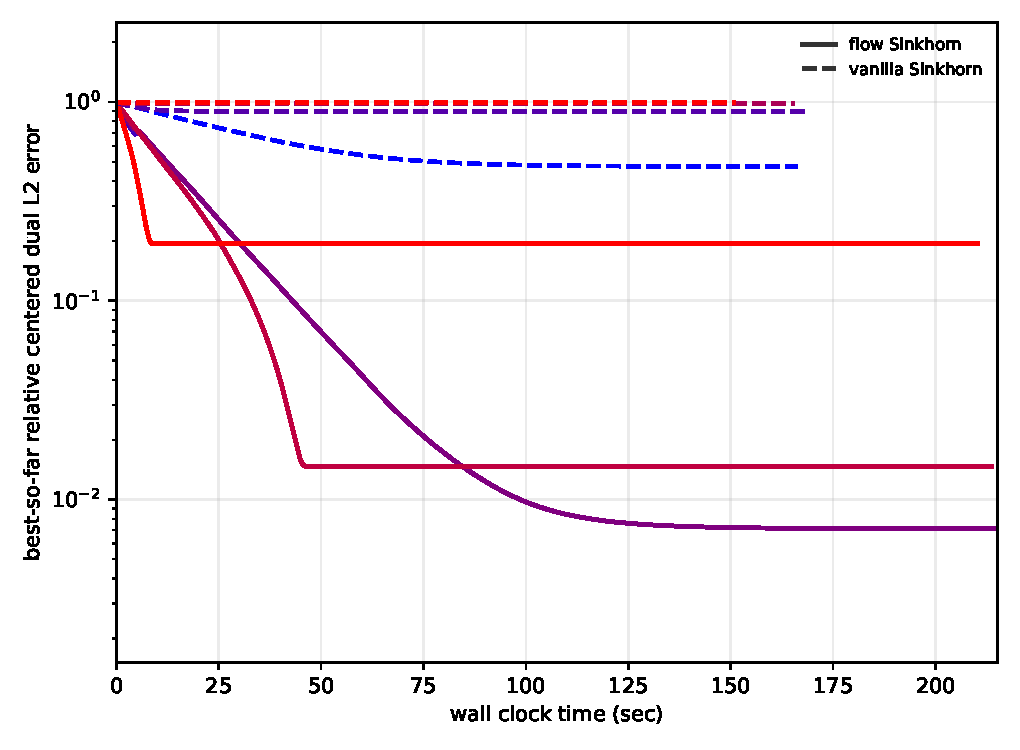
\includegraphics[width=\linewidth]{figures/benchmark-gpu-large-half-tuned-v2-line-convergence.pdf}
\end{minipage}\hfill
\begin{minipage}{0.32\linewidth}\centering
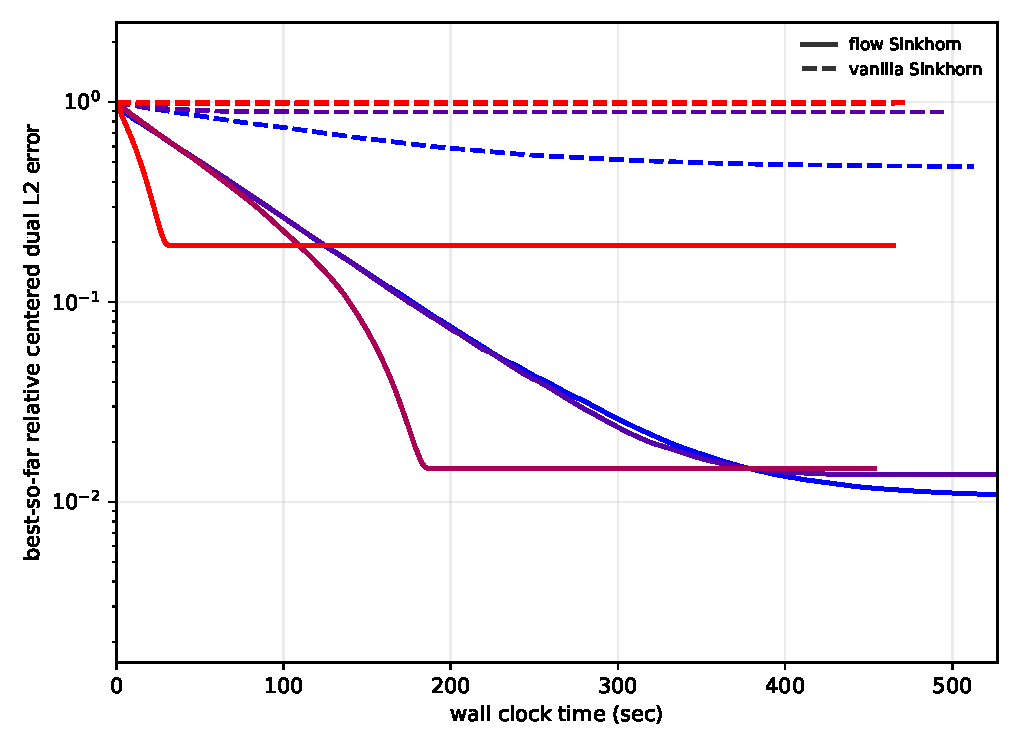
\includegraphics[width=\linewidth]{figures/benchmark-gpu-larger-half-tuned-v6-line-convergence.pdf}
\end{minipage}\vspace{-2mm}
\caption{GPU line-graph benchmark, same best-so-far relative centered dual-potential error as in Figure~\ref{fig:bench-overview-small}. From left to right: small ($n=80,m=6$), large ($n=160,m=12$), and larger ($n=320,m=24$) line-segment tests. %  Flow-Sinkhorn curves are solid and vanilla Sinkhorn curves are dashed.
}
\label{fig:bench-line-gpu-scaling}
\end{figure}

